\documentclass[9pt]{beamer}
\beamertemplatenavigationsymbolsempty
\usetheme{Berlin}

\usepackage{etex, tikz, array, graphics, xspace, relsize, multirow}
\usepackage{ulem}

\input binhex

% For code inclusion
\usepackage{listings}
\lstset{ breaklines=true}
\lstset{escapeinside={<@}{@>}}
\usepackage{algorithm2e}
\usepackage{algorithmic}

% Commands
\newcommand\A{\mathcal{A}}
\newcommand\cc{\mathcal{C}}
\newcommand\codim{\mathrm{codim}}
\newcommand\CP{\mathbb{CP}}
\newcommand\C{\mathbb{C}}
\newcommand\D{\mathrm{D}}
\newcommand\hto{\hookrightarrow}
\newcommand\I{^{-1}}
\newcommand\oo{\mathcal{O}}
\renewcommand\phi{\varphi}
\newcommand\Pj{\mathbb{P}}
\newcommand\pow{\mathcal{P}}
\newcommand\RP{\mathbb{RP}}
\newcommand\rstr[2]{{\left.#1\right|_{#2}}}
\newcommand\R{\mathbb{R}}
\newcommand\set[1]{\{#1\}}
\newcommand\toi{\xrightarrow{\sim}} % category
\newcommand\Z{\mathbb{Z}}


% For drawing
%% Tikz drawing
\usepackage{tikz}
\usetikzlibrary{arrows}
\usetikzlibrary{arrows.meta}
\usepackage{pgfplots}
\usepackage{tikz-3dplot}
\usepackage{tcolorbox}
\usetikzlibrary{matrix,fit,positioning,shapes.geometric,patterns,backgrounds}
\usetikzlibrary{decorations.pathreplacing}
\usetikzlibrary{decorations.markings}
\usetikzlibrary{arrows,calc}
\tikzstyle{bigbox} = [draw=blue!50, thick, rounded corners, rectangle]
\tikzset{
>=stealth'
}
\tikzset{->-/.style={decoration={
  markings,
  mark=at position #1 with {\arrow{>}}},postaction={decorate}}}

%% Software names
\newcommand\topcom{\texttt{TOPCOM}\xspace}
\newcommand\mptopcom{\texttt{MPTOPCOM}\xspace}
\newcommand\mptopcomone{\texttt{MPTOPCOM-1}\xspace}
\newcommand\mts{\texttt{mts}\xspace}
\newcommand\mplrs{\texttt{mplrs}\xspace}
\newcommand\soplex{\texttt{soplex}\xspace}
\newcommand\openmpi{\texttt{OpenMPI}\xspace}
\newcommand\mpi{\texttt{MPI}\xspace}
\newcommand\gfan{\texttt{Gfan}\xspace}
\newcommand\cddlib{\texttt{cddlib}\xspace}
\newcommand\polydb{\texttt{PolyDB}\xspace}
\newcommand\oscar{\texttt{OSCAR}\xspace}

\usepackage{xcolor}
\definecolor{green}{rgb}{0.1,0.59,0.1}
\definecolor{yellow}{rgb}{0.8,0.67,0}
\definecolor{red}{rgb}{0.89,0.1,0.1}
\definecolor{blue}{rgb}{0.1,0.1,0.89}

\usenavigationsymbolstemplate{}

\usepackage{booktabs}
% For software citations
\newcommand{\polymake}{\texttt{po\-ly\-ma\-ke}\xspace}
\newcommand{\polymakejl}{\texttt{Po\-ly\-ma\-ke.jl}\xspace}
\newcommand{\singular}{\texttt{Sin\-gu\-lar}\xspace}
\newcommand\CPP{C\nolinebreak\hspace{-.05em}\raisebox{.4ex}{\relsize{-3}{\textbf{+}}}\nolinebreak\hspace{-.10em}\raisebox{.4ex}{\relsize{-3}{\textbf{+}}}\xspace}

\usepackage{amsmath}
% Newcommands specifically for this article
\newcommand{\eval}{v}               % evaluation function giving switch table
\newcommand{\graph}{\Gamma}         % reverse search graph
\newcommand{\group}{G}              % group acting on point config
\newcommand{\groupElem}{g}          % element of group
\newcommand{\jbound}{\psi}          % bound on the number of elements of set J
\newcommand{\switchTableSize}{\mu}  % index of last non-trivial row in switch table

\newcommand{\pc}{\mathcal P\mathcal C}
\newcommand{\ZZ}{\mathbb Z}
\renewcommand{\AA}{\mathcal A}
\newcommand{\QQ}{\mathbb Q}
\newcommand{\OO}{\mathcal O}
\newcommand{\CC}{\mathbb C}
\newcommand{\PP}{\mathbb P}
\newcommand{\RR}{\mathbb R}
\newcommand{\scalp}[1]{\langle #1 \rangle}
\newcommand{\wt}{\omega}
\newcommand{\D}{\mathcal D}
\newcommand{\cT}{\mathcal T}
\renewcommand{\O}{\mathcal O}
\newcommand{\adm}{\mathcal A(\D, M)}
\newcommand{\blue}[1]{{\usebeamercolor[fg]{palette primary}#1}}

\DeclareMathOperator{\CaDiv}{CaDiv}
\DeclareMathOperator{\conv}{conv}
\DeclareMathOperator{\below}{defect}
\DeclareMathOperator{\vertex}{vertex}
\DeclareMathOperator{\Cox}{Cox}
\DeclareMathOperator{\cl}{cl}
\DeclareMathOperator{\cone}{cone}
\DeclareMathOperator{\Ext}{Ext}
\DeclareMathOperator{\Tor}{Tor}
\DeclareMathOperator{\lcm}{lcm}
\DeclareMathOperator{\Quot}{Quot}
\DeclareMathOperator{\Spec}{Spec}
\DeclareMathOperator{\Sets}{Sets}
\DeclareMathOperator{\relint}{relint}
\DeclareMathOperator{\rk}{rk}
\DeclareMathOperator{\smallestFace}{smallestFace}
\DeclareMathOperator{\Pic}{Pic}
\DeclareMathOperator{\Hom}{Hom}
\DeclareMathOperator{\vol}{vol}
\DeclareMathOperator{\TV}{TV}
\DeclareMathOperator{\tail}{tail}
\DeclareMathOperator{\rep}{rep}
\DeclareMathOperator{\vspan}{span}
\DeclareMathOperator{\canonical}{can}
\DeclareMathOperator{\gkz}{gkz}

\newcommand{\pmsmall}{
\includegraphics[scale=0.03]{pmlogo.png}}
\newcommand{\pmlogo}{
\includegraphics[scale=0.09]{pmlogo.png}}
\newcommand{\pmbluesmall}{\includegraphics[scale=0.03]{pmbluelogo.png}}
\newcommand{\Disjoint}{\mathop{\coprod}}
\newcommand{\Discriminant}{\mathcal{D}}

\theoremstyle{definition}
\newtheorem*{remark}{Remark}
\newtheorem*{lemma}{Lemma}
\newtheorem*{prop}{Proposition}
\newtheorem{defn}{Definition}

\author{Antony Della Vecchia}
\title{Computing Convex Hulls}
%\newtheorem*{example}{Example}
\institute[]{
Technische Universit\"at Berlin
}
\date{
2022-10-12
}


\newcommand{\surj}{\twoheadrightarrow}
\newcommand{\oursetting}[1]{\textcolor{blue}{#1}}
\usepackage{listings}
\begin{document}
\maketitle
%%%%%%%%%%%%%%%%%%%%%%%%%%%%%%%%%%%%%%%%%%%%%%%%%%%%%%%%%%%%%%%%%%%%%%%%%%%%%%%
%%%%%%%%%%%%%%%%%%%%%%%%%%%%%%%%%%%%%%%%%%%%%%%%%%%%%%%%%%%%%%%%%%%%%%%%%%%%%%%
%%%%%%%%%%%%%%%%%%%%%%%%%%%%%%%%%%%%%%%%%%%%%%%%%%%%%%%%%%%%%%%%%%%%%%%%%%%%%%%
\begin{frame}[fragile]{Overview}
  \begin{tcolorbox}
    \tableofcontents
  \end{tcolorbox}
\end{frame}
%%%%%%%%%%%%%%%%%%%%%%%%%%%%%%%%%%%%%%%%%%%%%%%%%%%%%%%%%%%%%%%%%%%%%%%%%%%%%%%
%%%%%%%%%%%%%%%%%%%%%%%%%%%%%%%%%%%%%%%%%%%%%%%%%%%%%%%%%%%%%%%%%%%%%%%%%%%%%%%
%%%%%%%%%%%%%%%%%%%%%%%%%%%%%%%%%%%%%%%%%%%%%%%%%%%%%%%%%%%%%%%%%%%%%%%%%%%%%%%

%%%%%%%%%%%%%%%%%%%%%%%%%%%%%%%%%%%%%%%%%%%%%%%%%%%%%%%%%%%%%%%%%%%%%%%%%%%%%%%
\section{Preliminaries}
%%%%%%%%%%%%%%%%%%%%%%%%%%%%%%%%%%%%%%%%%%%%%%%%%%%%%%%%%%%%%%%%%%%%%%%%%%%%%%%

\begin{frame}[fragile]{Hulls}
  \begin{defn}
    Let $A \subset \mathbb{K}^n$, an \emph{affine combination} of points in $A$
    is a linear combination $\sum_{i=1}^m \lambda_m a_m$ where $\lambda_m \in
    \mathbb{K}$ and $a \in A$ such that $\sum_{i=1}^m \lambda_m = 1$. The
    \emph{affine hull} is the set of all such combinations.
  \end{defn}

    \begin{defn}
    Let $A \subset \mathbb{R}^n$, a \emph{convex combination} of points in $A$
    is an affine combination $\sum_{i=1}^m \lambda_m a_m$ where $\lambda_m \geq
    0$. The  \emph{convex hull} is the set of all such combinations.
  \end{defn}

\end{frame}
%%%%%%%%%%%%%%%%%%%%%%%%%%%%%%%%%%%%%%%%%%%%%%%%%%%%%%%%%%%%%%%%%%%%%%%%%%%%%%%
%%%%%%%%%%%%%%%%%%%%%%%%%%%%%%%%%%%%%%%%%%%%%%%%%%%%%%%%%%%%%%%%%%%%%%%%%%%%%%%
%%%%%%%%%%%%%%%%%%%%%%%%%%%%%%%%%%%%%%%%%%%%%%%%%%%%%%%%%%%%%%%%%%%%%%%%%%%%%%%

\begin{frame}[fragile]{Polytopes}
  \begin{defn}
    A set $P \subset \mathbb{R}^n$ is a \emph{polytope} if it can be described
    as the convex hull of finitely many points. The dimension of $P$ is
    defined to be the dimension of it's affine hull. A \emph{$k$-polytope} is a
    k dimensional polytope. A \emph{$k$-simplex} is the convex hull of $k + 1$
    affine independant points.
  \end{defn}

  \begin{figure}
    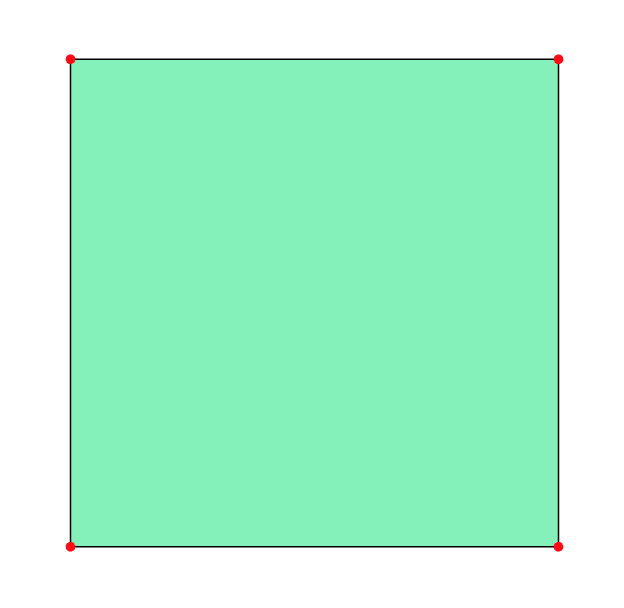
\includegraphics[width=.30\textwidth, height=0.4\textheight]{images/square}
    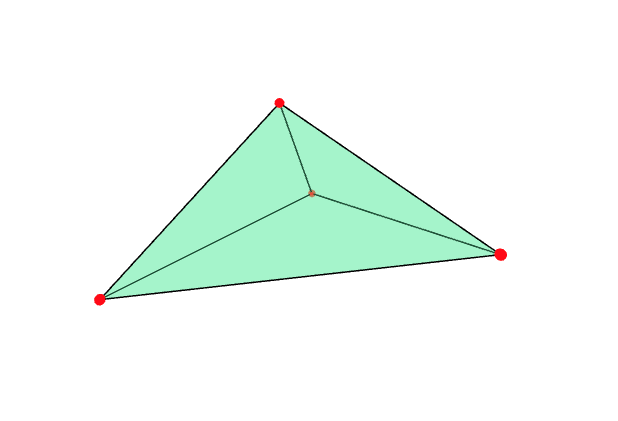
\includegraphics[width=.30\textwidth, height=0.4\textheight]{images/simplex}
  \end{figure}

\end{frame}
%%%%%%%%%%%%%%%%%%%%%%%%%%%%%%%%%%%%%%%%%%%%%%%%%%%%%%%%%%%%%%%%%%%%%%%%%%%%%%%
%%%%%%%%%%%%%%%%%%%%%%%%%%%%%%%%%%%%%%%%%%%%%%%%%%%%%%%%%%%%%%%%%%%%%%%%%%%%%%%
%%%%%%%%%%%%%%%%%%%%%%%%%%%%%%%%%%%%%%%%%%%%%%%%%%%%%%%%%%%%%%%%%%%%%%%%%%%%%%%


\begin{frame}[fragile]{Faces}
  \begin{defn}
    Given an n-polytope $P \subset \mathbb{R}^n$, the intersection $P \cap H$
    with a supporting hyperplane $H$ is called a \emph{proper face}. A face of
    dimension $k$ is called a $k$ face, a 0-face is a vertex, 1-face an edge,
    n-2 face a ridge and an n-1 face a facet.
  \end{defn}
  \begin{remark}
    Proper faces are also polytopes with respect to their affine hull.
  \end{remark}
  \begin{theorem}
    The boundary of a full dimesional polytope is the union of all it's
    proper faces.
  \end{theorem}

\end{frame}
%%%%%%%%%%%%%%%%%%%%%%%%%%%%%%%%%%%%%%%%%%%%%%%%%%%%%%%%%%%%%%%%%%%%%%%%%%%%%%%
%%%%%%%%%%%%%%%%%%%%%%%%%%%%%%%%%%%%%%%%%%%%%%%%%%%%%%%%%%%%%%%%%%%%%%%%%%%%%%%
%%%%%%%%%%%%%%%%%%%%%%%%%%%%%%%%%%%%%%%%%%%%%%%%%%%%%%%%%%%%%%%%%%%%%%%%%%%%%%%

\begin{frame}[fragile]{Half-spaces}
  \begin{defn}
    Given an affine hyperplane $H \subset \mathbb{R}^n$ given in homegeneous
    coordinates as $[a_0, \dots, a_n]$, define the \emph{positive halfspace}
    $H^+$ as $\{x \in \mathbb{R}^n \mid a_0 + a_1x_1 + \dots + a_nx_n \geq 0 \}$.
  \end{defn}

  \begin{remark}
    For each facet $f$ of a polytope $P$, there exists a positive halfspace $H^+$
    such that $f = P \cap H$ and $ P \subset H^+$
  \end{remark}

  \begin{center}
    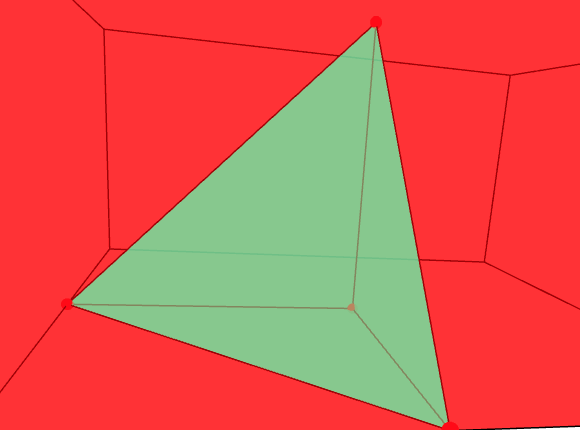
\includegraphics[width=.30\textwidth, height=0.4\textheight]{images/half-space}
  \end{center}
\end{frame}
%%%%%%%%%%%%%%%%%%%%%%%%%%%%%%%%%%%%%%%%%%%%%%%%%%%%%%%%%%%%%%%%%%%%%%%%%%%%%%%
%%%%%%%%%%%%%%%%%%%%%%%%%%%%%%%%%%%%%%%%%%%%%%%%%%%%%%%%%%%%%%%%%%%%%%%%%%%%%%%
%%%%%%%%%%%%%%%%%%%%%%%%%%%%%%%%%%%%%%%%%%%%%%%%%%%%%%%%%%%%%%%%%%%%%%%%%%%%%%%

\begin{frame}[fragile]{Polytope Descriptions}
  \begin{theorem}
    Let $H_i$ be the supporting hyperplanes for the facets of a polytope $P$.
    then $P = \cap_i^m H_i^+$
  \end{theorem}
  \begin{theorem}
    Every polytope is the convex hull of it's vertices
  \end{theorem}
  \begin{remark}
    Finding an algorithm for going between these descriptions is what will be
    interested in, and is what is meant by a convex hull computation.
  \end{remark}
\end{frame}
%%%%%%%%%%%%%%%%%%%%%%%%%%%%%%%%%%%%%%%%%%%%%%%%%%%%%%%%%%%%%%%%%%%%%%%%%%%%%%%
%%%%%%%%%%%%%%%%%%%%%%%%%%%%%%%%%%%%%%%%%%%%%%%%%%%%%%%%%%%%%%%%%%%%%%%%%%%%%%%
%%%%%%%%%%%%%%%%%%%%%%%%%%%%%%%%%%%%%%%%%%%%%%%%%%%%%%%%%%%%%%%%%%%%%%%%%%%%%%%

\begin{frame}[fragile]{Noteable Example}
  \begin{defn}
    The \emph{moment curve} $\mu_n \to \mathbb{R}^n$ is defined as
    $\tau \to (\tau, \dots, \tau^n)$. A polytope is called \emph{cyclic}
    if it is the convex hull of points on the moment curve.
  \end{defn}
  \begin{remark}
    Notice that since any $n + 1$ vertices lie in a distinct supporting
    hyperplane, that the number of facets is maximal given a fixed point
    of number vertices.
  \end{remark}

  \begin{center}
    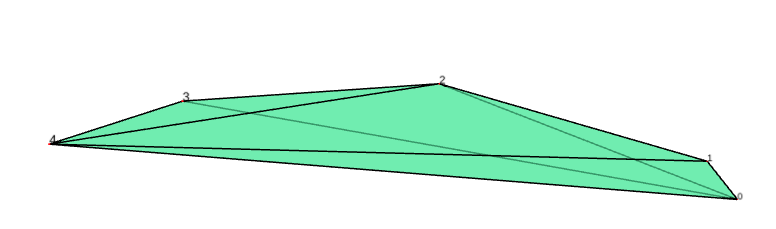
\includegraphics[width=.30\textwidth, height=0.4\textheight]{images/cyclic}
  \end{center}
\end{frame}
%%%%%%%%%%%%%%%%%%%%%%%%%%%%%%%%%%%%%%%%%%%%%%%%%%%%%%%%%%%%%%%%%%%%%%%%%%%%%%%
%%%%%%%%%%%%%%%%%%%%%%%%%%%%%%%%%%%%%%%%%%%%%%%%%%%%%%%%%%%%%%%%%%%%%%%%%%%%%%%
%%%%%%%%%%%%%%%%%%%%%%%%%%%%%%%%%%%%%%%%%%%%%%%%%%%%%%%%%%%%%%%%%%%%%%%%%%%%%%%

\begin{frame}[fragile]{Polarity and Duality}
  \begin{defn}
    Given a set $X \subset \mathbb{R}^n$ define the polar set as
    $X^o = \{y \in \mathbb{R}^n \mid x_1y_1 + \dots x_ny_n \leq 1\}$
  \end{defn}
  \begin{theorem}
    If $P \subset \mathbb{R}^n$ is an $n$-polytope with $0 \in \text{int}P$ then
    $P^o$ is also an $n$-polytope, and for $V$ the vertex set of $P$ we have
    \begin{center}
      $P^o = \bigcap_{v \in V} \set{y \in \R^n \mid \langle v, y \rangle \leq 1} = \bigcap_{v \in V} [1: -v_0: \dots : -v_n]^+$
    \end{center}
  \end{theorem}
  \begin{center}
    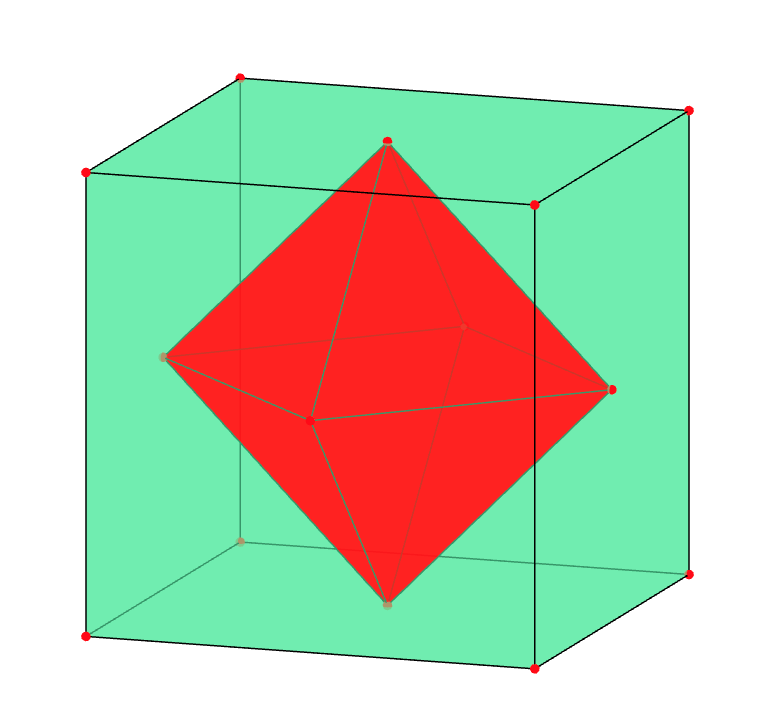
\includegraphics[width=.30\textwidth, height=0.4\textheight]{images/polar}
  \end{center}
\end{frame}
%%%%%%%%%%%%%%%%%%%%%%%%%%%%%%%%%%%%%%%%%%%%%%%%%%%%%%%%%%%%%%%%%%%%%%%%%%%%%%%
%%%%%%%%%%%%%%%%%%%%%%%%%%%%%%%%%%%%%%%%%%%%%%%%%%%%%%%%%%%%%%%%%%%%%%%%%%%%%%%
%%%%%%%%%%%%%%%%%%%%%%%%%%%%%%%%%%%%%%%%%%%%%%%%%%%%%%%%%%%%%%%%%%%%%%%%%%%%%%%

\begin{frame}[fragile]{Polarity and Duality}
  \begin{theorem}
    Let $P \subset \R^n$ be an $n$ polytope with $0 \in \text{int}P$ then
    \begin{itemize}
    \item $(P^o)^o = P$
    \item For any point $p$ on the boundary of $P$, $H = \set{x \in \R^n
      \mid \langle p, x \rangle = 1}$ is a supporting hyperplane of $P^o$
    \end{itemize}
  \end{theorem}
  \begin{remark}
    
  \end{remark}
  
\end{frame}
%%%%%%%%%%%%%%%%%%%%%%%%%%%%%%%%%%%%%%%%%%%%%%%%%%%%%%%%%%%%%%%%%%%%%%%%%%%%%%%
%%%%%%%%%%%%%%%%%%%%%%%%%%%%%%%%%%%%%%%%%%%%%%%%%%%%%%%%%%%%%%%%%%%%%%%%%%%%%%%
%%%%%%%%%%%%%%%%%%%%%%%%%%%%%%%%%%%%%%%%%%%%%%%%%%%%%%%%%%%%%%%%%%%%%%%%%%%%%%%

%%%%%%%%%%%%%%%%%%%%%%%%%%%%%%%%%%%%%%%%%%%%%%%%%%%%%%%%%%%%%%%%%%%%%%%%%%%%%%%
\section{Algorithms}
%%%%%%%%%%%%%%%%%%%%%%%%%%%%%%%%%%%%%%%%%%%%%%%%%%%%%%%%%%%%%%%%%%%%%%%%%%%%%%%

\begin{frame}[fragile]{A basic Algorithm}
  
  \begin{algorithm}[H]
    Input: Finite point set $V \subset \R^n$ with dimension of $\text{aff}V = n$\\
    Output: Finite set of half-spaces $H_i^+$ such that $\text{conv}(V) =
    \cap_{i=1}^m H_i^+$
    \begin{algorithmic}[1]
      \STATE $\mathcal{H}$ \leftarrow $\emptyset$
      \FOR{each $n$ element subset $W \subset V$ with dimension aff$W$}
      \STATE $H \leftarrow \text{aff} W$
      \IF{$V \subset H^+$}
      \STATE $\mathcal{H}$ \leftarrow $\mathcal{H} \cup H^+$
      \ELSE $\mathcal{H}$ \leftarrow $\mathcal{H} \cup H^-$
      \ENDIF
      \ENDFOR
      \RETURN $\mathcal{H}$
    \end{algorithmic}
  \end{algorithm}
\end{frame}
%%%%%%%%%%%%%%%%%%%%%%%%%%%%%%%%%%%%%%%%%%%%%%%%%%%%%%%%%%%%%%%%%%%%%%%%%%%%%%%
%%%%%%%%%%%%%%%%%%%%%%%%%%%%%%%%%%%%%%%%%%%%%%%%%%%%%%%%%%%%%%%%%%%%%%%%%%%%%%%
%%%%%%%%%%%%%%%%%%%%%%%%%%%%%%%%%%%%%%%%%%%%%%%%%%%%%%%%%%%%%%%%%%%%%%%%%%%%%%%

\begin{frame}[fragile]{A Partitioning Lemma}
  \begin{lemma}
    Let $V_0, V_+, V_-$ be the partition of a point set $V$,defined by
    $V_0 = V \cap H, V_+ = V \cap H^+ \setminus H, V_- = V \cap H^- \setminus H$
    where $H$ is a hyperplane. Then we have $P \cap H =
    \text{conv}(V_0 \cup V_+ \cup \set{[v, w] \cap H \mid v \in V_+ , w \in V_-})
  \end{lemma}
\end{frame}
%%%%%%%%%%%%%%%%%%%%%%%%%%%%%%%%%%%%%%%%%%%%%%%%%%%%%%%%%%%%%%%%%%%%%%%%%%%%%%%
%%%%%%%%%%%%%%%%%%%%%%%%%%%%%%%%%%%%%%%%%%%%%%%%%%%%%%%%%%%%%%%%%%%%%%%%%%%%%%%
%%%%%%%%%%%%%%%%%%%%%%%%%%%%%%%%%%%%%%%%%%%%%%%%%%%%%%%%%%%%%%%%%%%%%%%%%%%%%%%

\begin{frame}[fragile]{}
  \begin{algorithm}[H]
    Input: \\
    Output:
    \begin{algorithmic}[1]
      \FOR{$i=1$ to $N$}
      \FOR{$j=1$ to $JJJJ$}
      \STATE $energy[i*JJJ+j] =$ 
      $ interpolate(AAA[i*JJJ+j], ZZZ)$
      \ENDFOR
      \ENDFOR
    \end{algorithmic}
  \end{algorithm}
\end{frame}
%%%%%%%%%%%%%%%%%%%%%%%%%%%%%%%%%%%%%%%%%%%%%%%%%%%%%%%%%%%%%%%%%%%%%%%%%%%%%%%
%%%%%%%%%%%%%%%%%%%%%%%%%%%%%%%%%%%%%%%%%%%%%%%%%%%%%%%%%%%%%%%%%%%%%%%%%%%%%%%
%%%%%%%%%%%%%%%%%%%%%%%%%%%%%%%%%%%%%%%%%%%%%%%%%%%%%%%%%%%%%%%%%%%%%%%%%%%%%%%

\begin{frame}[fragile]{}
  blah
\end{frame}

%%%%%%%%%%%%%%%%%%%%%%%%%%%%%%%%%%%%%%%%%%%%%%%%%%%%%%%%%%%%%%%%%%%%%%%%%%%%%%%
%%%%%%%%%%%%%%%%%%%%%%%%%%%%%%%%%%%%%%%%%%%%%%%%%%%%%%%%%%%%%%%%%%%%%%%%%%%%%%%
%%%%%%%%%%%%%%%%%%%%%%%%%%%%%%%%%%%%%%%%%%%%%%%%%%%%%%%%%%%%%%%%%%%%%%%%%%%%%%%


%%%%%%%%%%%%%%%%%%%%%%%%%%%%%%%%%%%%%%%%%%%%%%%%%%%%%%%%%%%%%%%%%%%%%%%%%%%%%%%
\section{Remarks on Implementations}
%%%%%%%%%%%%%%%%%%%%%%%%%%%%%%%%%%%%%%%%%%%%%%%%%%%%%%%%%%%%%%%%%%%%%%%%%%%%%%%

\begin{frame}[fragile]{}
  blah
\end{frame}

%%%%%%%%%%%%%%%%%%%%%%%%%%%%%%%%%%%%%%%%%%%%%%%%%%%%%%%%%%%%%%%%%%%%%%%%%%%%%%%
%%%%%%%%%%%%%%%%%%%%%%%%%%%%%%%%%%%%%%%%%%%%%%%%%%%%%%%%%%%%%%%%%%%%%%%%%%%%%%%
%%%%%%%%%%%%%%%%%%%%%%%%%%%%%%%%%%%%%%%%%%%%%%%%%%%%%%%%%%%%%%%%%%%%%%%%%%%%%%%

\begin{frame}
  \frametitle{References}
  \footnotesize{
    \begin{thebibliography}{99} % Beamer does not support BibTeX so references must be inserted manually as below
    \bibitem[Joswig, Thorsten, 2013]{p1} Michael Joswig, Thorsten Theobald, (2013)
      \newblock Polyhedral and algebraic methods in computational geometry
      \newblock London: Springer

    \end{thebibliography}
  }
\end{frame}

%%%%%%%%%%%%%%%%%%%%%%%%%%%%%%%%%%%%%%%%%%%%%%%%%%%%%%%%%%%%%%%%%%%%%%%%%%%%%%%
%%%%%%%%%%%%%%%%%%%%%%%%%%%%%%%%%%%%%%%%%%%%%%%%%%%%%%%%%%%%%%%%%%%%%%%%%%%%%%%
%%%%%%%%%%%%%%%%%%%%%%%%%%%%%%%%%%%%%%%%%%%%%%%%%%%%%%%%%%%%%%%%%%%%%%%%%%%%%%%

\end{document}
